\documentclass[10pt,a4paper]{article}

\sloppy
\usepackage{caption}
\usepackage{subcaption}
\captionsetup{font = footnotesize, labelfont = bf}
\captionsetup[sub]{font=scriptsize,labelfont= bf}
\setlength{\textwidth}{16cm}
\setlength{\textheight}{23cm}
\addtolength{\hoffset}{-1.5cm}
\addtolength{\voffset}{-1.5cm}
\setlength{\headheight}{35pt}
\usepackage[utf8]{inputenc}
%\usepackage[spanish]{babel}
\usepackage[spanish,es-tabla]{babel}
\usepackage{ae}
\usepackage{graphicx}
\usepackage{wrapfig}
\usepackage{tikz,pgfplots}
\usepackage{epsfig}
%\usepackage{multicol, array}
\usepackage{amsmath}
\usepackage{amssymb, amsthm}
\usepackage{amsfonts}
\DeclareMathOperator\erf{erf}
%\theoremstyle{definition}
%\newtheorem*{definition}{Definición}
%\newtheorem*{example}{Ejemplo}
%\newtheorem*{theorem}{Teorema}
%\usepackage{epsdice}
\numberwithin{equation}{section}
\usepackage{euscript}
\usepackage{mathrsfs}
\usepackage{sectsty}
\usepackage{lipsum}
\usepackage{courier}
\usepackage{listings}
\usepackage{xcolor}
\definecolor{verde}{rgb}{0.0, 0.5, 0.1}

\lstset{
  language=R, literate =  {á}{{\'a}}1 {é}{{\'e}}1 {í}{{\'{\i}}}1 {ó}{{\'o}}1 {ú}{{\'u}}1 {Á}{{\'A}}1 {É}{{\'E}}1 {Í}{{\'I}}1 {Ó}{{\'O}}1 {Ú}{{\'U}}1 {ü}{{\"u}}1 {Ü}{{\"U}}1 {ñ}{{\~n}}1 {Ñ}{{\~N}}1,
  backgroundcolor=\color{gray!6!},
  classoffset=0,
  basicstyle=\ttfamily\small\bfseries,
  showspaces=false,
  showstringspaces=false,
  keywordstyle=\color{blue!60!black}\bfseries,
  stringstyle=\color{blue},
  numbers=none,
  numberstyle=\ttfamily\small,
  commentstyle=\color{verde}\textbf,
  morecomment=[l][\color{verde}\textbf],
  frame = single,
  framexleftmargin= -0pt,
  framexrightmargin= -5pt}


\usepackage{tcolorbox}
\tcbuselibrary{theorems}

\newtcbtheorem[auto counter,number within=section]{theorem}{Teorema}%
{colback=green!5,colframe=green!35!black,fonttitle=\bfseries}{th}

\newtcbtheorem[auto counter,number within=section]{definition}{Definición}%
{colback=blue!5,colframe=blue!35!black,fonttitle=\bfseries}{def}

\newtcbtheorem[auto counter,number within=section]{example}{Ejemplo}%
{colback=red!5,colframe=red!35!black,fonttitle=\bfseries}{ej}


%\newtcbtheorem[auto counter,number within=section]{theorem}{Teorema}%
%{colback=green!5,colframe=green!35!black,fonttitle=\bfseries}{th}

\newtcbtheorem[auto counter,number within=section]{software}{Software}%
{colback=yellow!5,colframe=yellow!35!black,fonttitle=\bfseries}{sw}

\usepackage{fancyhdr}

\decimalpoint
\usepackage[T1]{fontenc}
%\usepackage{textcomp}

\pagestyle{fancy}
\lhead{U.N.S.L. - Departamento de Física\\Lic. en Física - Física Experimental I}
%\rhead{
\includegraphics[width=0.8cm]{/home/juan/Documentos/Docencia/unsl.jpg}}
%\pagenumbering{arabic}
\rhead{
\includegraphics[width=0.8cm]{/home/juan/Documentos/Docencia/unsl.jpg}}

%\setcounter{page}{1}
\setlength{\parskip}{3mm}

\pgfplotsset{compat=1.13}

\usepackage{hyperref}
\hypersetup{
    colorlinks=true,
    linkcolor=blue,
    filecolor=black,      
    urlcolor=blue,
    citecolor=black,
   	anchorcolor=black
}
 
\urlstyle{same}

\begin{document}
\begin{center}
{
\begin{large}
\textbf{Laboratorio N$^o$ 6} \\
\vspace*{0.1cm}
\textbf{Una cuestión de dimensiones \linebreak (gráficas log-log)}

\end{large}
}
\end{center}





\medskip

\begin{flushright}
\begin{scriptsize}

``Ella me mira decorar el jarrón. En el jarrón pinto un jarrón, con flores, copia del jarrón sobre el que pinto. Para denotar la curvatura del jarrón que pinto, debo compensar la curvatura del jarrón sobre el que pinto. Desde luego, el jarrón que pinto debe incluir la figura de un jarrón, y para pintar este jarrón debo compensar las curvaturas del primero y del segundo. Es claro que este jarrón incluye a su vez otro y que para pintar su curvatura debiera compensar las curvaturas del primero, del segundo y del tercero, pero esto superaría mi capacidad. Así, aun cuando el observador -es decir ella, que me mira- no pueda percibirlo, el cuarto jarrón es en verdad deforme y puede decirse, no que represente pero sí que figura el campo de mi deformidad. ''


Pedro Lipcovich\footnote{Escritor argentino nacido en Buenos Aires (1950). Libros publicados: El nombre verdadero (1989), Muñecos chicos (El cuenco de plata, 2005), Unas polillas (2009). Obtuvo el Primer Premio del Fondo Nacional de las Artes 2009. Por el cuento \textit{redaliz} (incluido en Unas polillas) recibió el Premio Internacional de Cuento ``Juan Rulfo'', otorgado por el Centro Cultural de México en París y Radio Francia Internacional.}. Muñecos Chicos (2005), El Cuenco de Plata Ed. 

\end{scriptsize}
\end{flushright}

\section{Introducción}

\subsection{Dimensión Topológica}
La etimología de la palabra \textit{dimensión} nos remite a un concepto largamente estudiado en Física Experimental, ya que viene del latín $d\bar{i}mensi\bar{o}$, abstracto de $d\bar{e}m\bar{e}tiri$, ``medir''. Sin embargo, a primera vista, en matemáticas, la idea de dimensión no tiene mucho que ver con la física experimental: la dimensión de un conjunto o \textit{espacio topológico}, está caracterizada por la \textit{topología} (del griego \textit{$\tau$\hspace*{-0.5mm}ó$\pi o \varsigma$} --topos--  'lugar, superficie', y $\lambda$ó$\gamma o \varsigma$ --logos--, 'estudio').

Entrar en detalle no sólo es engorroso, sino que en este caso es inaccesible (la topología no es materia simple). La idea de dimensión topológica está asociada a la idea de \textit{cubierta} --conjuntos pequeños que \textit{recubren  el conjunto cuya dimensión queremos determinar}-- y da por resultado un número entero, que es $0$ para el punto, $1$ para una línea, $2$ para una superficie, $3$ para un volumen...los espacios topológicos o conjuntos pueden ser entonces $0-dimensonal$, $1-dimensonal$, $2-dimensonal$, $3-dimensonal$,..., $n-dimensonal$.

\subsection{Medida (en matemáticas)}
Al estudiar las medidas (aquí propondremos las conocidas, longitud, área, volumen) de conjuntos, veremos que la dimensión aparece sin tantos tecnicismos. Ponemos en consideración:

\begin{itemize}
\item[\textbf{i)}] Un segmento $S$ de longitud $a$.
\item[\textbf{ii)}] Un rectángulo $R$ de lados con longitud $a,b$, respectivamente.
\item[\textbf{iii)}] Un paralelepípedo $P$ de lados cuya longitud es $a,b,c$., respectivamente 
\end{itemize}

Para los conjuntos anteriores, ponemos en consideración las medidas $m(S)$, $m(R)$ y $m(P)$, definidas como:
\begin{itemize}
\item[\textbf{i)}] $m(S) = a$, es decir, la longitud del segmento $S$.
\item[\textbf{ii)}] $m(R) = ab$, es decir, el área del rectángulo $R$.
\item[\textbf{iii)}] $m(P) = abc$, es decir, el volumen del paralelepípedo $P$.
\end{itemize}

\subsection{Medidas de conjuntos semejantes, relación con la dimensión del conjunto}

Imaginemos que multiplicamos por un factor real $k$ (con $0 < k < \infty$) los conjuntos $S$, $R$ y $P$ vistos anteriormente. Con la multiplicación por $k$, tenemos un segmento semenjante $S' = kS$ (una obviedad, porque todos los segmentos son semejantes), un rectángulo semejante $R' = kR$ y un paralelepípedo semejante $P' = kP$. Ahora, ¿cómo varían las medidas luego de la multiplicación por $k$? Tenemos:

\begin{itemize}
\item[\textbf{i)}] $m(S') = m(kS) =  ka = k\;m(S)$, es decir, la longitud del segmento $S'$ es $k$ veces la longitud de $S$.
\item[\textbf{ii)}] $m(R') = m(kR) = (ka)(kb) = k^2 ab = k^2 \; m(R)$, es decir, el área del rectángulo $R'$ es $k^2$ veces el área de $R$.
\item[\textbf{iii)}] $m(P') = m(kP) = (ka)(kb)(kc) = k^3 abc = k^3 \; m(P)$, es decir, el volumen del paralelepípedo $P'$ es $k^3$ veces el volumen de $P$.
\end{itemize}

\noindent lo anterior puede generalizarse de la siguiente manera, dado un conjunto $A' = kA$, entonces la medida sobre el conjunto, $m(kA)$ queda:

\begin{equation}\label{edim}
m(kA) = k^D m(A)
\end{equation}

\noindent donde en la ec.\eqref{edim}, $D$ es la dimensión del conjunto. Dadas las nociones familiares (aunque no estudiadas) de topología, $D$ es un valor entero que adopta los valores $D = 0,1,2,3,4,...$. 


\section{Sobre la longitud de la costa de Inglaterra}

\begin{wrapfigure}{r}{0.525\linewidth}
\vspace*{-8mm}
\begin{center}
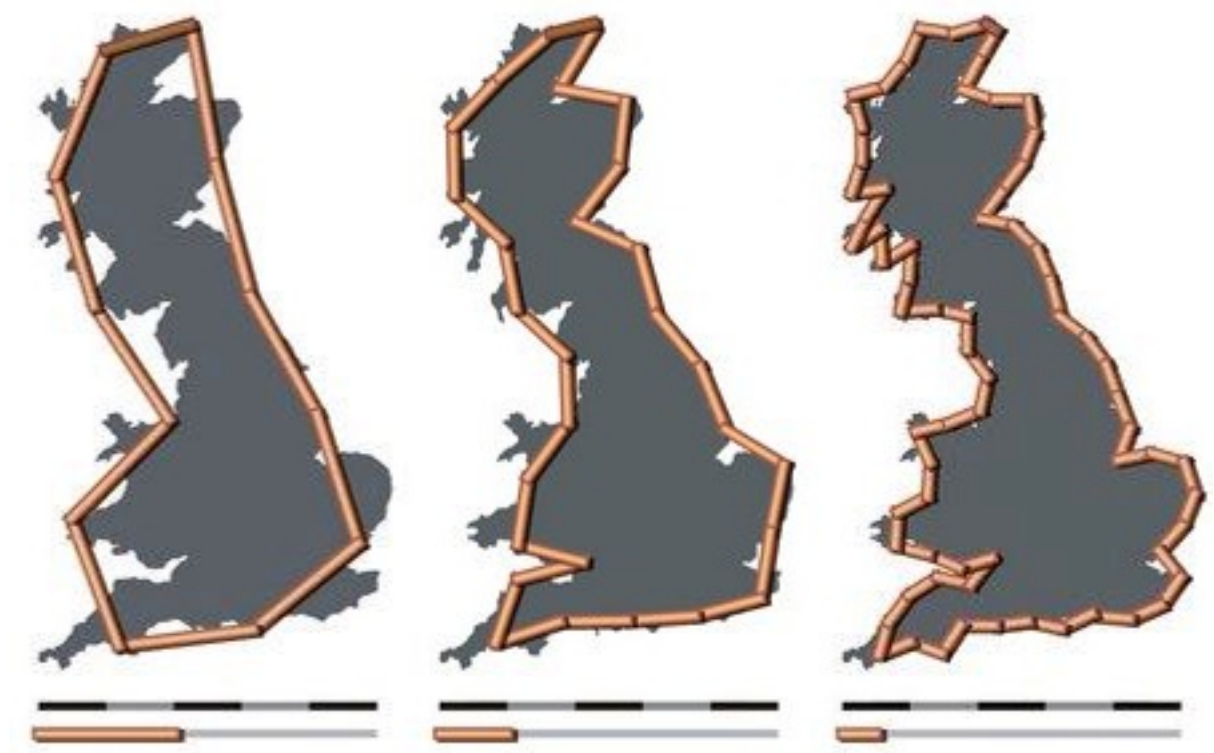
\includegraphics[width=1\linewidth]{costa.png}
\vspace*{-5mm}
\caption{Costa de Gran Bretaña recubierta con pasos menores cada vez. Fuente: \textit{García Fernández, E.}, ``Teoría de la Dimensión Topológica''. Tesis, U. Cantabria. 2018.}
\label{fcosta}
\vspace*{10mm}
\end{center}
\end{wrapfigure}

La costa de Inglaterra\footnote{Utilizamos la de Inglaterra por razones históricas, razones que, tal vez, podrían habernos llevado a elegir islas más cercanas, como las Islas Malvinas.} puede ser considerada una línea ($D = 1$), que delimita Inglaterra. Medir una costa no es tarea sencilla, y hay diferentes versiones a lo largo de la historia de la geografía. Un primer problema a la hora de medir longitudes de costa reside en que la línea costera es muy \textit{quebrada} o \textit{poco suave}, con lo que deberemos explicitar un método (no podremos decir que medimos la longitud de la costa con una cinta métrica). Una de las posibildades --entre muchas otras equivalentes--, es recorrer la costa con segmentos de largo $\eta$, hasta cubrirla completamente, como puede verse en la Fig.(\ref{fcosta}). Luego de cubrir toda la costa, entonces tenemos que el largo de la costa es $L(\eta) = m \eta$, donde $m$ es el número de círculos que utilizamos.

\href{https://es.wikipedia.org/wiki/Lewis_Fry_Richardson}{Lewis Fry Richardson} fue un científico que, mientras miraba diferentes enciclopedias, cayó en la cuenta de que las longitudes informadas para ciertas fronteras eran \textit{demasiado} diferentes en los distintos textos. Richardson recopiló toda la información disponible sobre las costas, froteras y medidas. Una gráfica de la recopilación de datos puede verse en la Fig.\eqref{frichardson}, donde se muestra la longitud de diferentes entes geográficos (froteras, costas, y...un círculo) en escala logarítmica \textit{vs.} el largo de los \textit{segmentos} utilizados para cubrir las longitudes (también es escala logarítmica). Observando los resultados de la gráfica, Richardson extrajo la siguiente relación entre $L$, la longitud total del ente geográfico y el largo del segmento utilizado para medir $\eta$:

\begin{equation}\label{er}
log(L) = a - b \; log(\eta) 
\end{equation}

\noindent donde la ec. \eqref{er}, tiene las constantes $a, b$ y relaciona el logaritmo del largo del ente geográfico $log(L)$ con el logaritmo del paso utilizado para medirlo, $log(\eta)$. 

La ec.\eqref{er} puede obtenerse en forma lineal como:
\begin{equation}\label{erl}
L = A \eta^{-b} 
\end{equation}

\begin{itemize}
\item[$\bullet$] Calcular la constante $A$ de la ec.\eqref{erl} en función de las constantes de la ec.\eqref{er}.
\item[$\bullet$] Evaluar los límites de $L$ para $\eta \rightarrow 0$ y $\eta \rightarrow \infty$.
\end{itemize}


Fue \href{https://es.wikipedia.org/wiki/Beno\%C3\%AEt_Mandelbrot}{Mandelbrot} quien evaluó que el problema mostrado por Richardson obedecía a una problemática general: ¿realmente podemos considerar a una costa o curva fracturada \textit{ad-nauseam} un ente de dimensión 1? ¿o es posible considerar que una curva muy \textit{quebrada} tiene una dimensión mayor?


\begin{figure}[t!] 
\begin{center}
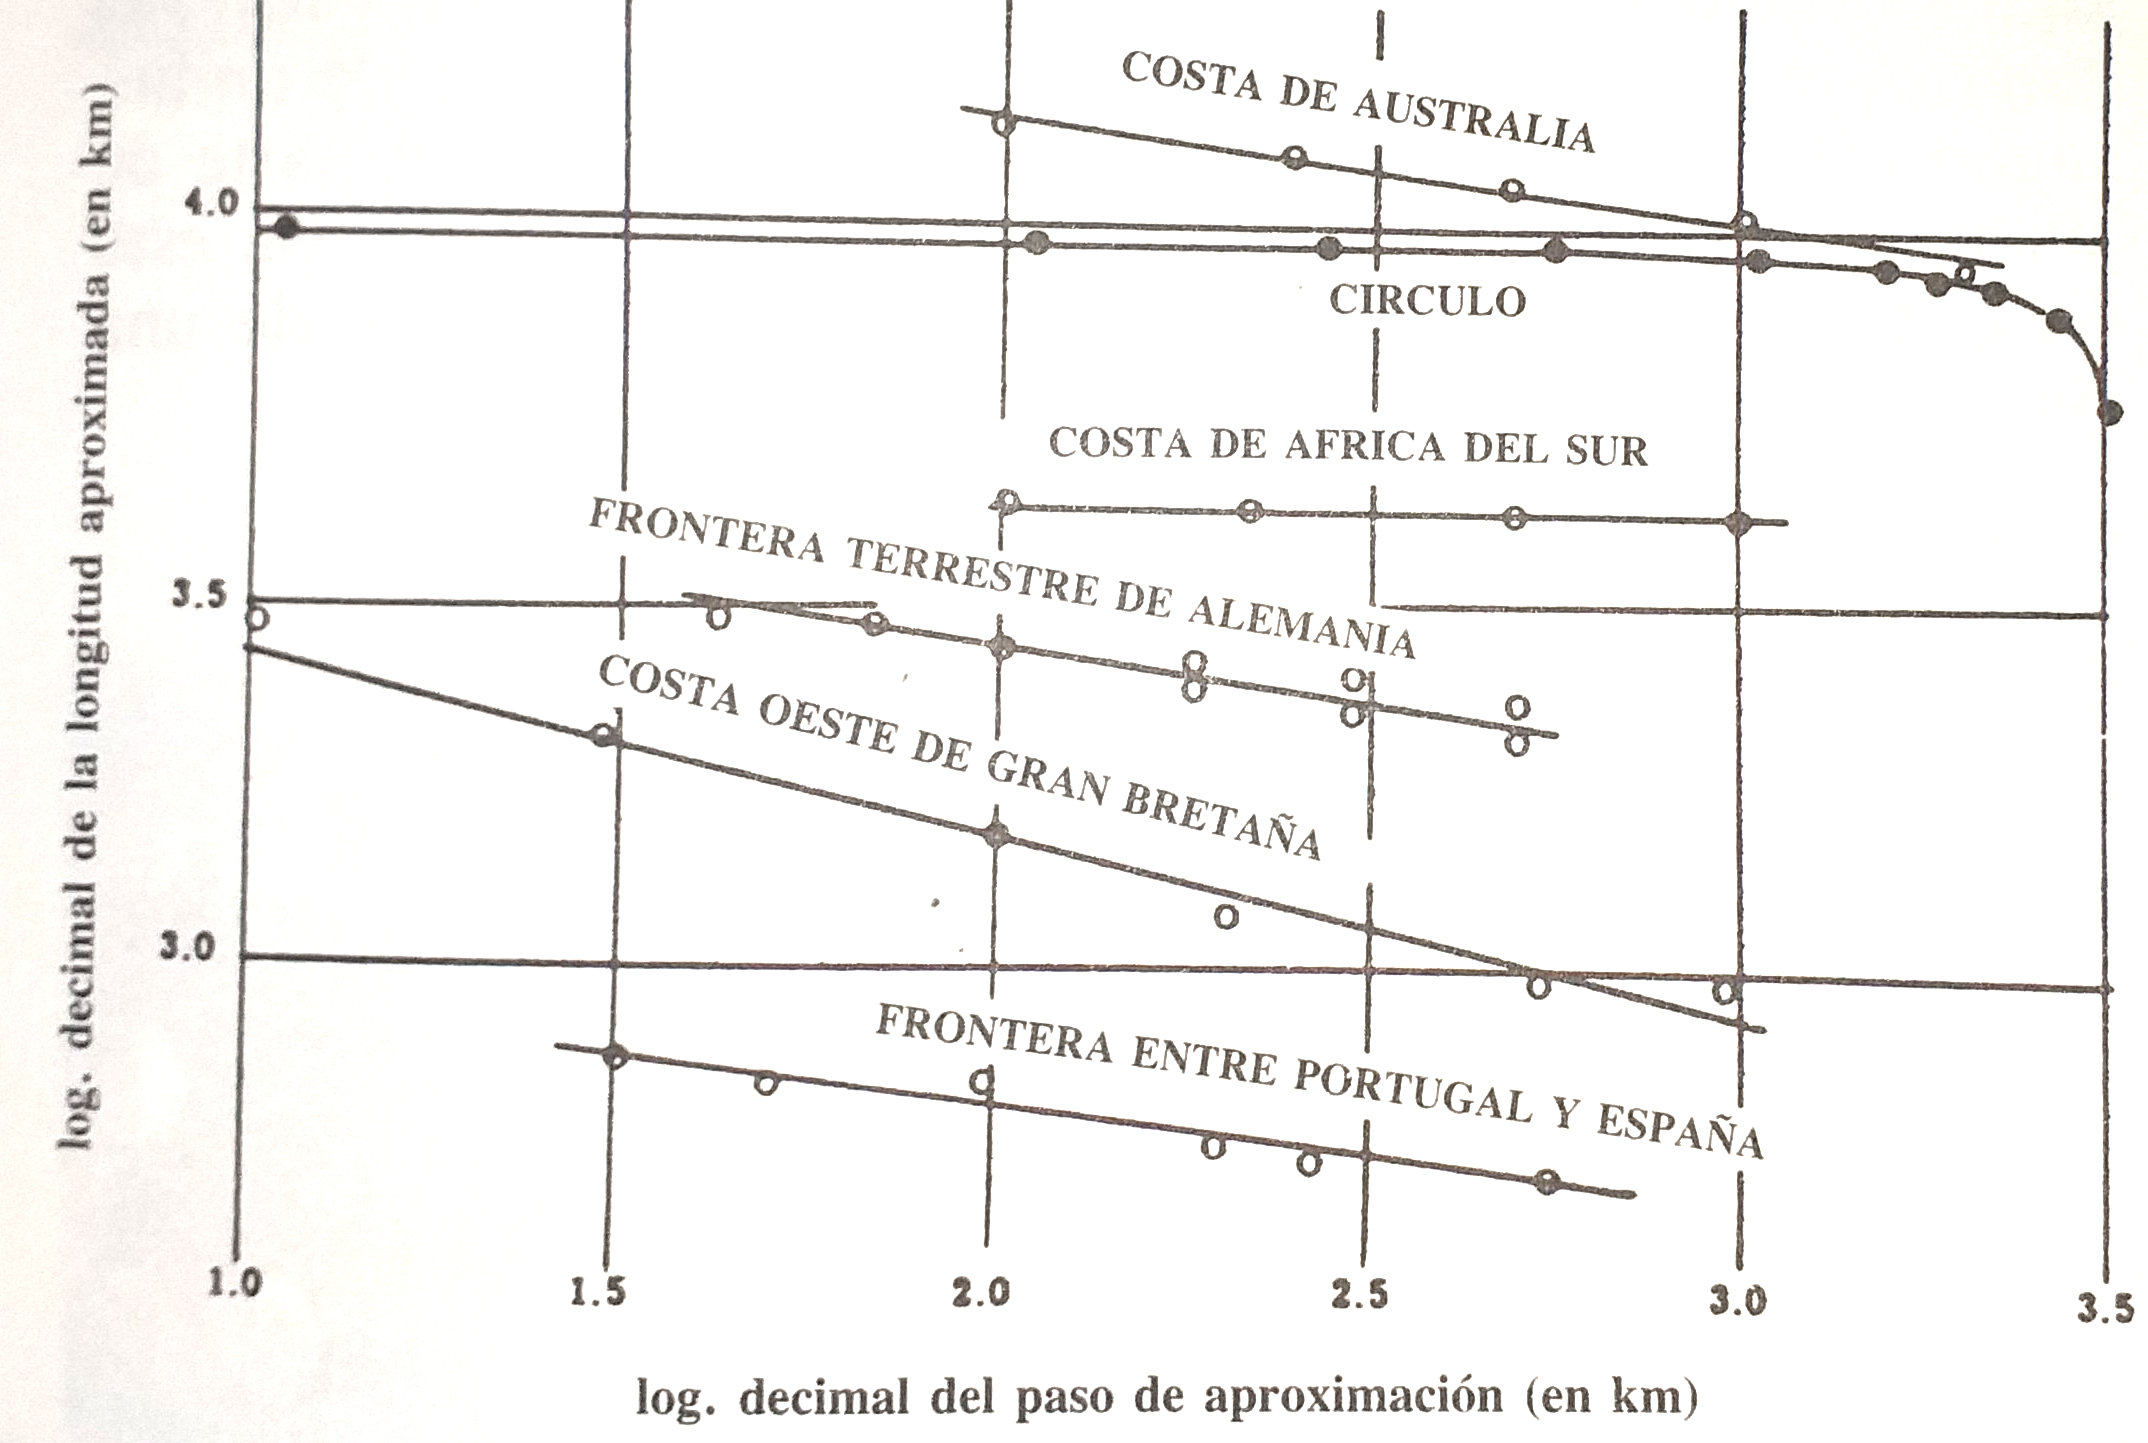
\includegraphics[width=100mm]{costasrichardson.jpg}
\caption{Longitudes de diferentes costas, recopiladas por \href{https://es.wikipedia.org/wiki/Lewis_Fry_Richardson}{Lewis Fry Richardson} y exhumadas por Mandelbrot en ``Los objetos Fractales'' (1984) Tusquets Ed.}
\label{frichardson}
\end{center}
\end{figure}

\pagebreak
\subsection{Curva de Koch o un modelo matemático para las costas}

\begin{figure}[htb!] 
\begin{center}
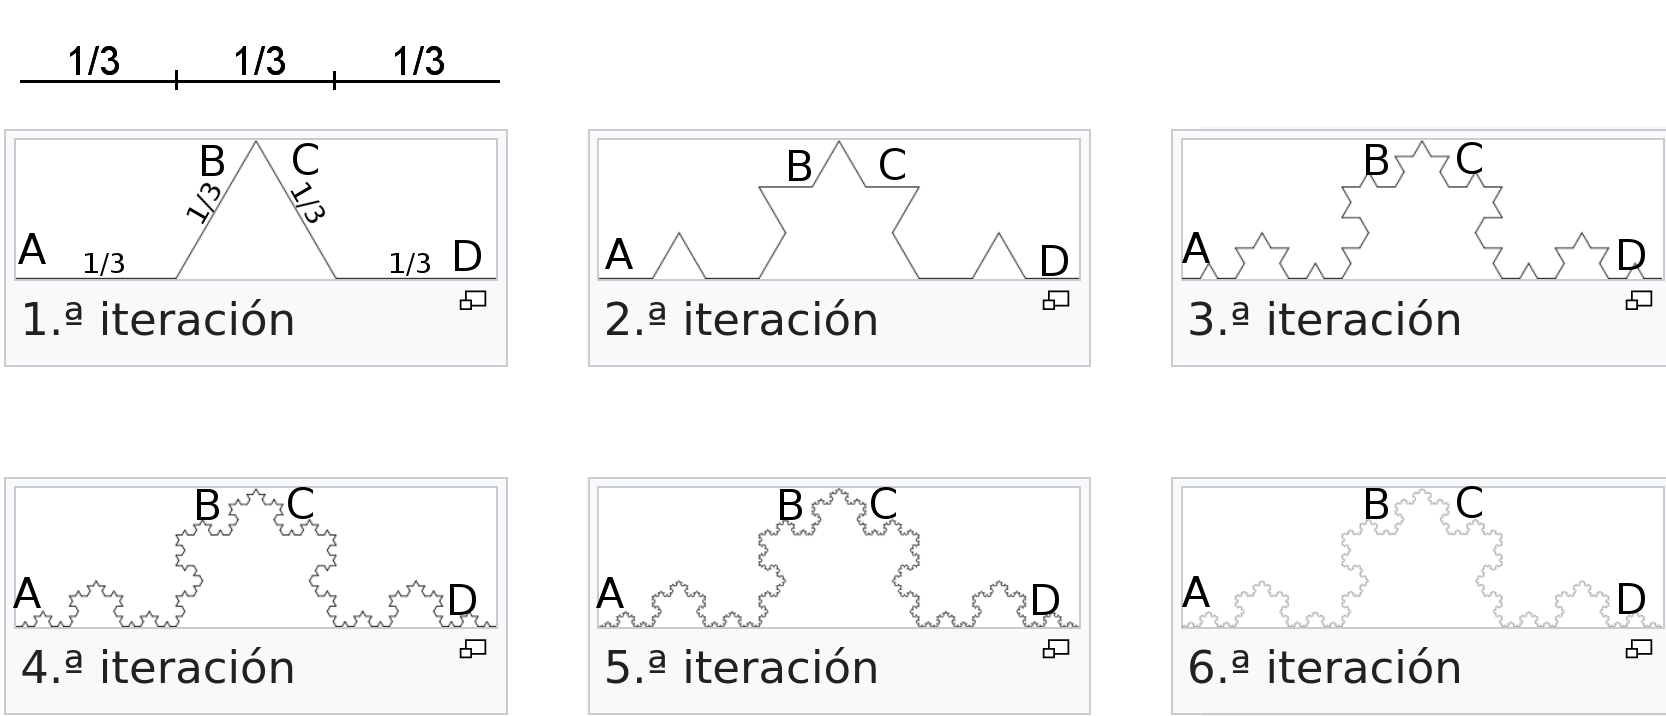
\includegraphics[width=145mm]{flKoch.png}
\caption{Proceso Iterativo que lleva a la línea de Koch, partiendo de un segmento de longitud $l$: (a).Todo segmento recto de longitud $a$ se divide en tres partes iguales, de longitudes $a/3$. (b). En la parte central de las divisiones anteriores se le agrega un cuarto segmento de longitud $a/3$ y se realiza un triángulo equilátero. Repetir (1) y (2) infinitas veces entrega la curva de Koch, que Koch buscaba como ejemplo de línea contínua y no suave en ningún punto. Fuente: Christophe Dang Ngoc Chan, trabajo propio en Wikipedia.}
\label{flkoch}
\end{center}
\end{figure}

Una curva de Koch es una curva geométrica que se obtiene por iteración. Como puede verse en la Fig.\eqref{flkoch}, partiendo de un segmento de longitud $l$:
\begin{itemize}
\item[\textbf{(i)}] Se parte en tres partes iguales de longitud $l/3$.
\item[\textbf{(ii)}] Se agrega una porción de longitud $l/3$ para formar un triángulo equilátero en la porción central.
\end{itemize}


\noindent para obtener la curva de Koch, las operaciones \textbf{(i)} y \textbf{(ii)} se repiten infinitas veces, sobre todas los segmentos generados.

La curva de Koch tiene algunas propiedades:
\begin{itemize}
\item[(a)] No tiene derivada en ningún punto a pesar de ser perfectamente continua, es decir, está \textit{infinitamente quebrada} (era la propiedad buscada por von Koch).
\item[(b)] Es \textit{autosimilar} entre ciertas partes y el todo: el proceso iterativo utilizado para formarla, hace que el primer tercio horizontal (descrito por $A$ en la Fig.\eqref{flkoch}) \textit{estirado o aumentado} en un factor $k = 3$ sea \textit{igual} a a \textit{curva entera}.
\item[(c)] Las partes $A, B,C,D$ tienen la misma \textit{medida}, es decir $m(A)=m(B)=m(C)=m(D)$, pues todas parten de $l/3$ y se construyen de la misma manera.
\end{itemize}

\noindent las propiedades anteriores nos permiten afirmar que, llamando $K$ a la curva de Koch (y siendo que $K$ es la unión de $A,B,C,D$)\footnote{$K = A \cup B \cup C \cup D$}:

\noindent  Según la propiedad (b), multiplicar el trecho $A$ por $k = 3$ es \textit{igual} a la curva de Koch $K$, esto es, la parte $A$ es semejante con $K$. Si seguimos las relaciones de la dimensionalidad expresada en la ec.\eqref{edim}:

\begin{equation}\label{edk}
m(K) = k^D m(A) = 3^D m(A)
\end{equation}

\noindent Por otra parte, la medida de toda la curva $K$ es la suma de sus partes:
\begin{equation}\label{esuma}
m(K) = m(A) + m(B) + m(C) + m(D) 
\end{equation}

\noindent y por a propiedad (c) que dice que $m(A) = m(B) = m(C) = m(D)$, podemos escribir:
\begin{equation}\label{e4x}
m(K) =4 \;m(A)
\end{equation}

\noindent igualando las ecs.\eqref{e4x} \eqref{edk}, podemos calcular la dimensión $D$ de la curva de Koch, como:

 \begin{align}\label{edimk}
 m(K) &= m(K) \Rightarrow \nonumber \\
 3^D m(A)  &= 4 \; m(A)  \Rightarrow \nonumber \\
 log(3^D) &= log(4) \Rightarrow \nonumber \\
 D &= \frac{log(4)}{log(3)} = log_3(4) \sim 1.261859507142915... 
 \end{align}

\noindent lo cual sería una locura sino fuera porque ya sabemos el desenlace: una nueva geometría, la geometría fractal, descubierta a partir de diferentes ideas de dimensión, que revolucionó varias áreas de investigación en el S. XX, constituída a partir de fragmentos dispersos, juntados por Mandelbrot (que es el apellido de Benoît, pero también un \href{https://www.thespruceeats.com/jewish-mandelbrot-recipe-1136149}{bizcocho de almendras}, típico de la comida ashkenazi).

La curva de von Koch es un ejemplo de costa, es decir, de una línea \textit{tan quebrada} ó \textit{fracturada}\footnote{Fracturada nos remite a fractal, que Mandelbrot eligió deliberadamente del latín (\textit{fractus, a, um}), quiere decir literalmente quebrado, fracturado. Nada más desagradable que las personas pedantes que van por las etimologías.} que tiene una \textit{dimensión fractal o efectiva}\footnote{Sin entrar en detalles, igualamos términos desiguales} diferente de la dimensión topológica entera.

\begin{itemize}
\item[$\bullet$] Calcule el largo de la curva de von Koch.
\end{itemize} 


\subsection{Dimensiones fractales}

Las dimensiones fractales \textit{pueden} adoptar valores reales en lugar de enteros. Geométricamente hablando, y por simplificar, miden cuán quebrada está una línea, una superficie, o un volumen, y el resultado es que las dimensiones fractales, por lo general (y salvando casos patológicos que también existen), son mayores que la dimensión topológica del conjunto en cuestión, es decir, hablamos de líneas con dimensión fractal $D_f > 1$, de superficies con $D_f > 2$ y de volúmenes con $D_f > 3$. 

Este tipo de dimensión está presente en muchas ramas de la física, de diferentes maneras: a veces aparece como una construcción teórica (similar a la curva de von Koch) y otras aparece a partir de los datos (similar a las costas). 

\pagebreak
\section{Actividad: Dimensiones fractales en esferas de papel}
La idea básica es medir \textit{empaquetamiento} de esferas (es un decir) de papel. Para ello utilizaremos:

\begin{itemize}
\item[$\bullet$] Dos hojas A4 por estudiante. Los tamaños utilizados por cada estudiante serán: una hoja entera; $1/2$ hoja, $1/4$ de hoja y $1/8$ de hoja (que repetirá dos veces). Cada estudiante compactará los papeles de los distintos tamaños a mano, intentando formar algo similar a una esfera.
\item[$\bullet$] Un calibre (mediremos con la escala de $mm$, la longitud de una esfera de papel no está indeterminada por la escala), con el cual tomaremos $n = 6$ medidas de diámetro por esfera construída de masa $m$
\item[$\bullet$] Una balanza para medir la masa.
\end{itemize}

\subsection{Sobre la organización de Datos}

Los datos tendrán el formato \textit{tidy}, usual, con las columnas:

\noindent \texttt{masa, diámetro, nombre}

Obviamente, tendremos seis medidas de diámetro por cada masa (la cual mediremos sólo una vez por esfera).

Los datos serán compartidos en la red, para todo el curso.

\section{Cuentas y análisis}



\subsection*{Para \textit{cada} estudiante}

Vamos a cargar los datos \textit{individuales} de las 5 esferas de cada estudiante. Es claro que tenemos 5 masas $m$ diferentes y al menos 6 radios $r$ por cada masa. Los radios dispares pueden pensarse com una variable $r$ no está \textit{definida}, es decir, la \textit{esfera} no es perfecta.

Casi todos los gráficos que vamos a hacer tienen en el eje vertical el radio $r$: como vamos a hacer ajustes, es necesario que la variable con mayor dispersión esté en el eje vertical (es un detalle no menor de los ajustes).

Lo que nos guiará es buscar una dimensión fractal $D$ a partir de la relación entre el radio y la masa de las esferas construídas. Es claro que la vamos a obtener de datos experimentales, por lo que tendremos una $D \pm \sigma_D$ (lo que en los modelos como la curva de Koch es un número real, a nosotros nos dará una distribución)


\noindent \textbf{0)}  Realice:
\begin{itemize}
\item[$\bullet$] El cálculo del volumen $V$ de las esferas para cada radio $r$ obtenido.
\item[$\bullet$] El cálculo de la \textit{densidad volumétrica} $\rho$ de las esferas a partir de la masa $m$ y el volumen $V$.
\item[$\bullet$] El gráfico de la densidad volumétrica $\rho$ vs. la masa $m$. 
\item[$\bullet$] El gráfico de la densidad volumétrica $\rho$ vs. el radio $r$. 
\end{itemize}

\begin{itemize}
\item[a)] ¿La densidad volumétrica es constante en las diferentes masas o radios?
\item[b)] Escriba un modelo, de densidad volumétrica constante $\rho$, que vincule los radios $r$ con las masas $m$ de esferas, es decir, obtenga una ecuación $r(m)$ para $D = 3$.
\end{itemize}


\-----------------------------------

\noindent \textbf{1)} Grafique el radio $r$ de las esferas vs. la masa $m$ de las esferas:

\begin{itemize}
\item[a)] ¿Qué relación deberían tener en el caso en el que la densidad volumétrica $\rho$ fuera constante para todas las esferas de papel?
\item[b)] Exprese $log(r)$ como función de $log(m)$ en la ec. obtenida en (0.b).
\item[c)] Escriba una ecuación que sea $r(m)$, utilizando una dimensión arbitraria $D_f$ (puede utilizar una constante de proporcionalidad A).
\end{itemize}


\-----------------------------------

\noindent \textbf{2)} Realice:

\begin{itemize}
\item[$\bullet$] Un gráfico del logaritmo del radio de las esferas vs. el logaritmo de la masa de las esferas. 
\item[$\bullet$] Realice un ajuste lineal en los datos anteriores.
\end{itemize} 


\begin{itemize}
\item[a)] Evalúe el gráfico en forma cualitativa ¿Los datos parecen \textit{linealizarse}?
\item[b)]  Identifique parámetros del ajuste lineal con la ecuación escrita en (1.c). Obtenga una dimensión fractal $D_f \pm \sigma_{D_f}$. ¿La distribución obtenida, está \textit{cerca} de un número entero, por ejemplo 2 ó 3 ?
\end{itemize}

Encontramos hasta ahora la dimensión fractal de una superficie muy abigarrada, quebrada, fracturada (la hoja de papel). Evalúe el valor obtenido contrastándolo con las ideas discutidas.



\subsection*{Otras inquisiciones grupales}

\noindent \textbf{3)} Haga una tabla con los resultados de todo el curso de $D_f \pm \sigma_{D_f}$. ¿Quién comprime más las esferas? Explicar detenidamente.

\-----------------------------------\


\noindent \textbf{4)} Grafique los volúmenes $V$ \textit{vs.} de los radios $r$.

\begin{itemize}
\item[a)] Escriba una función $V(r)$ que describa los datos.
\item[b)] Encuentre los parámetros necesarios mediante un ajuste lineal.
\end{itemize}

Ojo con graficar relaciones a partir de cálculos: la estructura que aparece es la cuenta que hicimos, y no tiene un pelo de experimental.

\-----------------------------------\

\noindent \textbf{4)} Grafique las densidades volumétricas $\rho$ \textit{vs.} el radio $r$. ¿Qué está ocurriendo? Puede hacer el tamaño de punto proporcional a las masas. Haga el mismo gráfico pero con escala doble logarítmica.

\-----------------------------------\\

\noindent \textbf{5)} Haga medias de los radios de cada esfera. Repita el gráfico anterior con estos datos. Repiense los resultados y vuelva a responder. Haga el gráfico en escala doble logarítmica.

Cuando hacemos cálculos, muchas veces las ecuaciones usadas dan estructuras que no están en los datos originales...siempre es mejor extraer conclusiones de los datos originales.

\-----------------------------------

\noindent \textbf{6)} Grafique en escala doble logarítmica $r$ vs. $m$ para todo el curso. Realice un ajuste lineal. Informe parámetros. Vea el residuo del ajuste ¿Cuál es el rango en el que se mueven los radios respecto del ajuste?

\end{document}